% -*- latex -*-
%%%%%%%%%%%%%%%%%%%%%%%%%%%%%%%%%%%%%%%%%%%%%%%%%%%%%%%%%%%%%%%%
%%%%%%%%%%%%%%%%%%%%%%%%%%%%%%%%%%%%%%%%%%%%%%%%%%%%%%%%%%%%%%%%
%%%%
%%%% This text file is part of the source of 
%%%% `Parallel Programming in MPI and OpenMP'
%%%% by Victor Eijkhout, copyright 2012-2020
%%%%
%%%% ddt_course.tex : master file for a lecture on debugging
%%%%
%%%%%%%%%%%%%%%%%%%%%%%%%%%%%%%%%%%%%%%%%%%%%%%%%%%%%%%%%%%%%%%%
%%%%%%%%%%%%%%%%%%%%%%%%%%%%%%%%%%%%%%%%%%%%%%%%%%%%%%%%%%%%%%%%

\documentclass[11pt,headernav]{beamer}

\beamertemplatenavigationsymbolsempty
%\usetheme{TACC16}
\usetheme{Madrid}%{Montpellier}
\usecolortheme{seahorse}
\setcounter{tocdepth}{1}

\setbeamertemplate{footline}{\hskip1em Eijkhout: Debugging intro\hfill
  \hbox to 0in {\hss 
\includegraphics[scale=.1]{tacclogonew}}%
  \hbox to 0in {\hss \arabic{page}\hskip 1in}}

\input commonmacs
\input slidemacs
\input coursemacs
\input listingmacs

\def\Location{}% redefine in the inex file
\def\Location{TACC/XSEDE training 2021}
\def\TitleExtra{}

%%%%
%%%% Where is this course?
%%%%

\def\Location{}% redefine in the inex file
\def\courseyear{2021}
\def\Location{TACC HPC Training \courseyear}

\includecomment{full}
\excludecomment{condensed}
\excludecomment{online}

\specialcomment{tacc}{\stepcounter{tacc}\def\CommentCutFile{tacc\arabic{tacc}.cut}}{}
\newcounter{tacc}
%\excludecomment{tacc}
\excludecomment{xsede}
\includecomment{utonly}

\includecomment{onesided}
\includecomment{advanced}
\includecomment{foundations}

\begin{xsede}
  \def\Location{TACC/XSEDE MPI training \courseyear}
\end{xsede}
\def\TitleExtra{}

%%%%%%%%%%%%%%%%
%%%%%%%%%%%%%%%% Document
%%%%%%%%%%%%%%%%

\begin{document}
\parskip=10pt plus 5pt minus 3pt

\title{Tutorial on Parallel Debugging}
\author{Victor Eijkhout}
\date{\Location}

\begin{frame}
  \titlepage
\end{frame}

\begin{frame}[containsverbatim]{Defensive programming}
  \begin{itemize}
  \item
    Better than finding errors is peventing them:\\
    defensive programming.
    \item One possibility:
      Use `assertions' about things that have to be true.
  \end{itemize}

  \lstset{language=C}
\begin{lstlisting}
#include <assert.h>
// for C++: #include <cassert>
assert( x>= 0 );
y = sqrt(x)
\end{lstlisting}

\begin{itemize}
\item
  Program will terminate if the assertion fails.
\item Disable assertions in production by defining \n{NDEBUG}
\end{itemize}

\end{frame}


\begin{frame}[containsverbatim]{Compiling for debug}
Enable debug mode with \n{-g} option:
\begin{verbatim}
mpicc -g -O2 yourprogram
\end{verbatim}
Debug option can be used with any optimization level, but
sometimes good to start at \n{-O0}:
\begin{verbatim}
mpicc -g -O0 yourprogram
\end{verbatim}
Compiler optimizations may confuse you otherwise.
\end{frame}

\begin{frame}[containsverbatim]{Important! Note! About! Exercises!}
  \begin{enumerate}
  \item You should have a directory \n{exercises_ddt_c} (or maybe~\n{f}).
    Go there.
  \item Start an interactive session: \n{idev}
  \item Exercise slides will have a program name at the top: \n{[roots]}.\\
    This means you compile with \n{make roots}
  \item Run your program with \n{./roots} if sequential\\
    or \n{ibrun roots} for parallel.
  \end{enumerate}
\end{frame}

\sectionframe{Traditional sequential debugging}

\begin{frame}{Debugging approaches}
  \begin{itemize}
  \item Print statements:
    \begin{itemize}
    \item can be effective, but they often perturb the behaviour:\\
      crashing code mysteriously works with print statements.
    \item Also: the error is often not where you think it is.
    \item Lots of recompilation.
    \end{itemize}
  \item Interactive debuggers, different approaches:
    \begin{enumerate}
    \item Start program in debugger
    \item Attach debugger to running program
    \item Do `post mortem' analysis on `core dump'.
    \end{enumerate}
  \end{itemize}
\end{frame}

\begin{frame}[containsverbatim]{Interactive debuggers}
  \begin{itemize}
  \item Commandline based tools:\\
    \n{gdb} comes free with Gnu compilers; other debuggers are very
    similar\\
    (Apple has switched to \n{lldb}, which has different commands)
  \item Graphic frontends: Visual Studio, CLion, Eclipse, Xcode,~\ldots
  \end{itemize}

  \begin{itemize}
  \item Catch interrupts and inspect state of the program
  \item Interrupt a run yourself to inspect variables (breakpoints)
  \item Step through a program.
  \end{itemize}
\end{frame}

\begin{frame}[containsverbatim]{Example}
  \begin{itemize}
  \item
    Compile \n{roots.c}: \n{make roots}
  \item 
    Run the program, first on the commandline. Output?
  \item Execute this sequence of commands:
    \begin{itemize}
    \item \n{gdb root}
    \item \n{run}, observe the output
    \item \n{quit}
    \end{itemize}
  \end{itemize}
\end{frame}

\begin{frame}[containsverbatim]{Diagnosing the problem}
  \begin{itemize}
  \item Floating point errors do not stop your program!
  \item In the debugger type:
    \begin{itemize}
    \item \n{break roots.c:32} or whatever the first line of the
      \n{root} function is
    \item \n{run} and note that it stops at the break point.
    \item \n{where} displays the `stack frames'; \n{frame 3} to go there
    \item \n{list} shows you the sources around the breakpoint
    \item \n{print n} to show your the current value
    \item \n{cont} to continue execution.
    \end{itemize}
  \item Better: \n{break roots.c:32 if (n<0)}
  \end{itemize}
\end{frame}

\begin{frame}{More gdb}
  \begin{tabular}{|l|l|}
    \hline
    command&meaning\\
    \hline
    \texttt{run / cont}&start~/ continue \\
    \texttt{break file.c:123}&breakpoint at line\\
    \texttt{break <location> if <condition>}&conditional stop\\
    \texttt{delete 1 / enable 2 / disable 3}&break point manipulation\\
    \texttt{where}&show call stack\\
    \texttt{frame 2}&specific frame\\
    \hline
  \end{tabular}

  For more commands see the cheat sheet in the course package.
\end{frame}

\begin{exerciseframe}[roots]
  You can force your execution to stop at floating point errors:\\
  \n{feenableexcept}\\
  Uncomment that line in the source, compile and run program,
  both commandline and debugger.\\
  In the debugger, inspect the offending line in all frames.
\end{exerciseframe}

\begin{frame}[containsverbatim]{Everyone's favourite error: memory problems}
  \begin{itemize}
  \item Write outside the bounds of an array\\
    (runtime checks are too expensive)
  \item Write to unallocated memory
  \item Read from unitialized memory.
  \end{itemize}
  First two can usually be caught with a debugger;\\
  third one: use a memory tool like \n{valgrind}
\begin{tacc}
\begin{verbatim}
module load valgrind
\end{verbatim}
\end{tacc}

\begin{verbatim}
valgrind myprogram # sequential
ibrun valgrind myprogram # parallel
\end{verbatim}
\end{frame}

\begin{exerciseframe}[array1]
  Compile and run \n{array1.c}.\\
  (Look in the source to see the problem.)\\
  If the program does not crash, recompile:
\begin{verbatim}
make clean array1 EXTRA_OPTIONS=5000
\end{verbatim}
or even more.
\end{exerciseframe}

\begin{frame}[containsverbatim]{Memory tools: valgrind}
  \begin{itemize}
  \item At TACCP \n{module load valgrind}
  \item run with \n{valgrind array1}
  \item Look at the diagnostics. Do you understand them?
  \end{itemize}
\end{frame}

\begin{frame}[containsverbatim]{Same program in the debugger}
  \small
\begin{verbatim}
Program received signal SIGSEGV, Segmentation fault.
0x0000000000400b31 in main (argc=1, argv=0x7fffffff95a8) at array1.c:33
33          squares[i] = 1./(i*i);
Missing separate debuginfos, use: debuginfo-install glibc-2.17-260.el7_6.3.x86_64
(gdb) where
#0  0x0000000000400b31 in main (argc=1, argv=0x7fffffff95a8) at array1.c:33
(gdb) print i
$1 = 5784
(gdb) print squares
$2 = (float *) 0x7fffffff95a0
\end{verbatim}
After a while you `get a feel' for what is a legitimate address
and what is not. This is not.
\end{frame}

\begin{exerciseframe}[array2]
  Access out of bounds.
  Can you find the problem with the debugger or with valgrind?

  Bonus exercise: what does valgrind say if you remove the 
  initialization of \n{sum}?
\end{exerciseframe}

\sectionframe{Parallel debugging}

\begin{frame}[containsverbatim]{Your minimal parallel debugger}
\begin{verbatim}
mpirun -np 4 xterm -e gdb yourprogram
\end{verbatim}
Pops up 4 xterms.\\
Great for debugging on your laptop.\\
Not great at scale.
\end{frame}

\begin{frame}{The DDT debugger}
  Originally by Allinea, now bought by ARM.
  \begin{itemize}
  \item Graphical front-end to gdb-like and valgrind-like capabilities
  \item Some specifically parallel features
  \item Commercial, and with very few open source alternatives\\
    (Eclipse with PTP)
  \item An absolute life-saver!
  \end{itemize}
\end{frame}

\begin{frame}[containsverbatim]{Using the DDT debugger}
  Load the module:
\begin{verbatim}
module load ddt
\end{verbatim}
Call the debugger:
\begin{verbatim}
ddt yourprogram
\end{verbatim}

\end{frame}

\begin{frame}[containsverbatim]{Graphics on a TACC cluster}
  \begin{itemize}
  \item
    Through an X forwarding connection:
\begin{verbatim}
ssh -X you@stampede.tacc.utexas.edu
\end{verbatim}
\item  use VNC.
\item use DCV
  (\url{https://portal.tacc.utexas.edu/tutorials/remote-desktop-access}):
\begin{verbatim}
# submit DCV job:
sbatch /share/doc/slurm/job.dcv
# when the job is running:
cat dcvserver.out
\end{verbatim}
The \n{dcvserver.out} file contains a URL: this gives a graphical terminal session
in your browser.
  \end{itemize}
\end{frame}

\begin{frame}{DDT modes}
  \begin{itemize}
  \item Start on login node, let DDT submit to queue\\
    you may need to wait a little while
  \item Start on compute node, DDT runs directly, not through queue
  \item Also `reverse connect' and batch mode, see
    \url{https://portal.tacc.utexas.edu/tutorials/ddt}
  \end{itemize}
\end{frame}

\begin{frame}[containsverbatim]{Run parameters}
  \begin{multicols}{2}
    \includegraphics[scale=.3]{runsubmit}
    \columnbreak
    \begin{itemize}
    \item MPI or OpenMP? Processes, nodes, threads.
    \item Memory debugging
    \item Commandline arguments
    \item Check `submit' when running on a login node:\\
      it submits to the queue for you;\\
      uncheck if starting from idev session.
    \end{itemize}
  \end{multicols}
\end{frame}

\begin{frame}[containsverbatim]{Submission setup}
  \begin{multicols}{2}
    \includegraphics[scale=.3]{queue}
    \columnbreak
    \begin{itemize}
    \item Project: your own, or one for this class
    \item Queue: development often quickest
    \end{itemize}
  \end{multicols}
\end{frame}

\begin{frame}[containsverbatim]{}
  \includegraphics[scale=.4]{init}
  \begin{itemize}
  \item Program starts at \n{MPI_Init}
  \item Use run controls
  \end{itemize}
\includegraphics[scale=.4]{controls}
\end{frame}

\begin{frame}[containsverbatim]{Hanging processes}
  \includegraphics[scale=.4]{hang}
  \begin{itemize}
  \item Red: stopped at an interrupt or breakpoint
  \item Green: still running.\\
    All green but `nothing happening': probably hanging program.
  \item Combination: some processes are not getting to the breakpoint:
    probably deadlocked.
  \end{itemize}
\end{frame}

\begin{frame}[containsverbatim]{Call stacks}
  \includegraphics[scale=.4]{stopped}
  \begin{itemize}
  \item Hit the pause button, go to `stacks' panel.
  \item Not every process is in the same source line.
  \item Click on process number to see what it's doing.
  \end{itemize}
\end{frame}

\begin{frame}[containsverbatim]{Breakpoints}
  \includegraphics[scale=.35]{breakpoint}
  \begin{itemize}
  \item Set breakpoint by clicking left of the line
  \item when you run, it will stop at the breakpoint.
  \end{itemize}

  \begin{itemize}
  \item Values display: everyone the same \n{it}
  \item value of \n{mytid} linearly increasing
  \item value of \n{randomnumber} all over the place.
  \end{itemize}
\end{frame}

\begin{exerciseframe}[finalize]
  Compile and run \n{finalize.c}.\\
  Every process completes the run, yet the program is incorrect.
  \begin{itemize}
  \item Uncomment the barrier command and rerun. What do you observe?
  \item Set a breakpoint inside the conditional. Do all processes reach it?
  \end{itemize}
\end{exerciseframe}

\begin{exerciseframe}[bcast]
  Compile and run \n{bcast.c}.\\
  The program finishes, yet it is not correct. (Why?)

  Recompile:
\begin{verbatim}
make clean
make bcast EXTRA_OPTIONS=-DN=100000
\end{verbatim}
  Does the program still complete?
\end{exerciseframe}

\begin{exerciseframe}[sendrecv1]
  Another program that is incorrect, but that
  finishes because small messages slip through the network.

  Replace \n{MPI_Send} with \n{MPI_Ssend} which enforces blocking behavior.\\
  Now what happens?
\end{exerciseframe}

\begin{exerciseframe}[sendrecv2]
  This code fixes the problem with \n{sendrecv1}.\\
  But is this sensible?

  \begin{itemize}
  \item \n{module load tau}
  \item Compile with TAU:\\
    \n{make clean; make sendrecv2}
  \item Run and generate trace files:\\
    \n{make taurun PROGRAM=sendrecv2}
  \item Postprocess:\\
    \n{make tau PROGRAM=sendrecv2}
  \item Somewhere with X windows:\\
    \n{jumpshot tautrace_sendrecv2.slog2}
  \end{itemize}
\end{exerciseframe}

\begin{frame}{TAU visualization}
  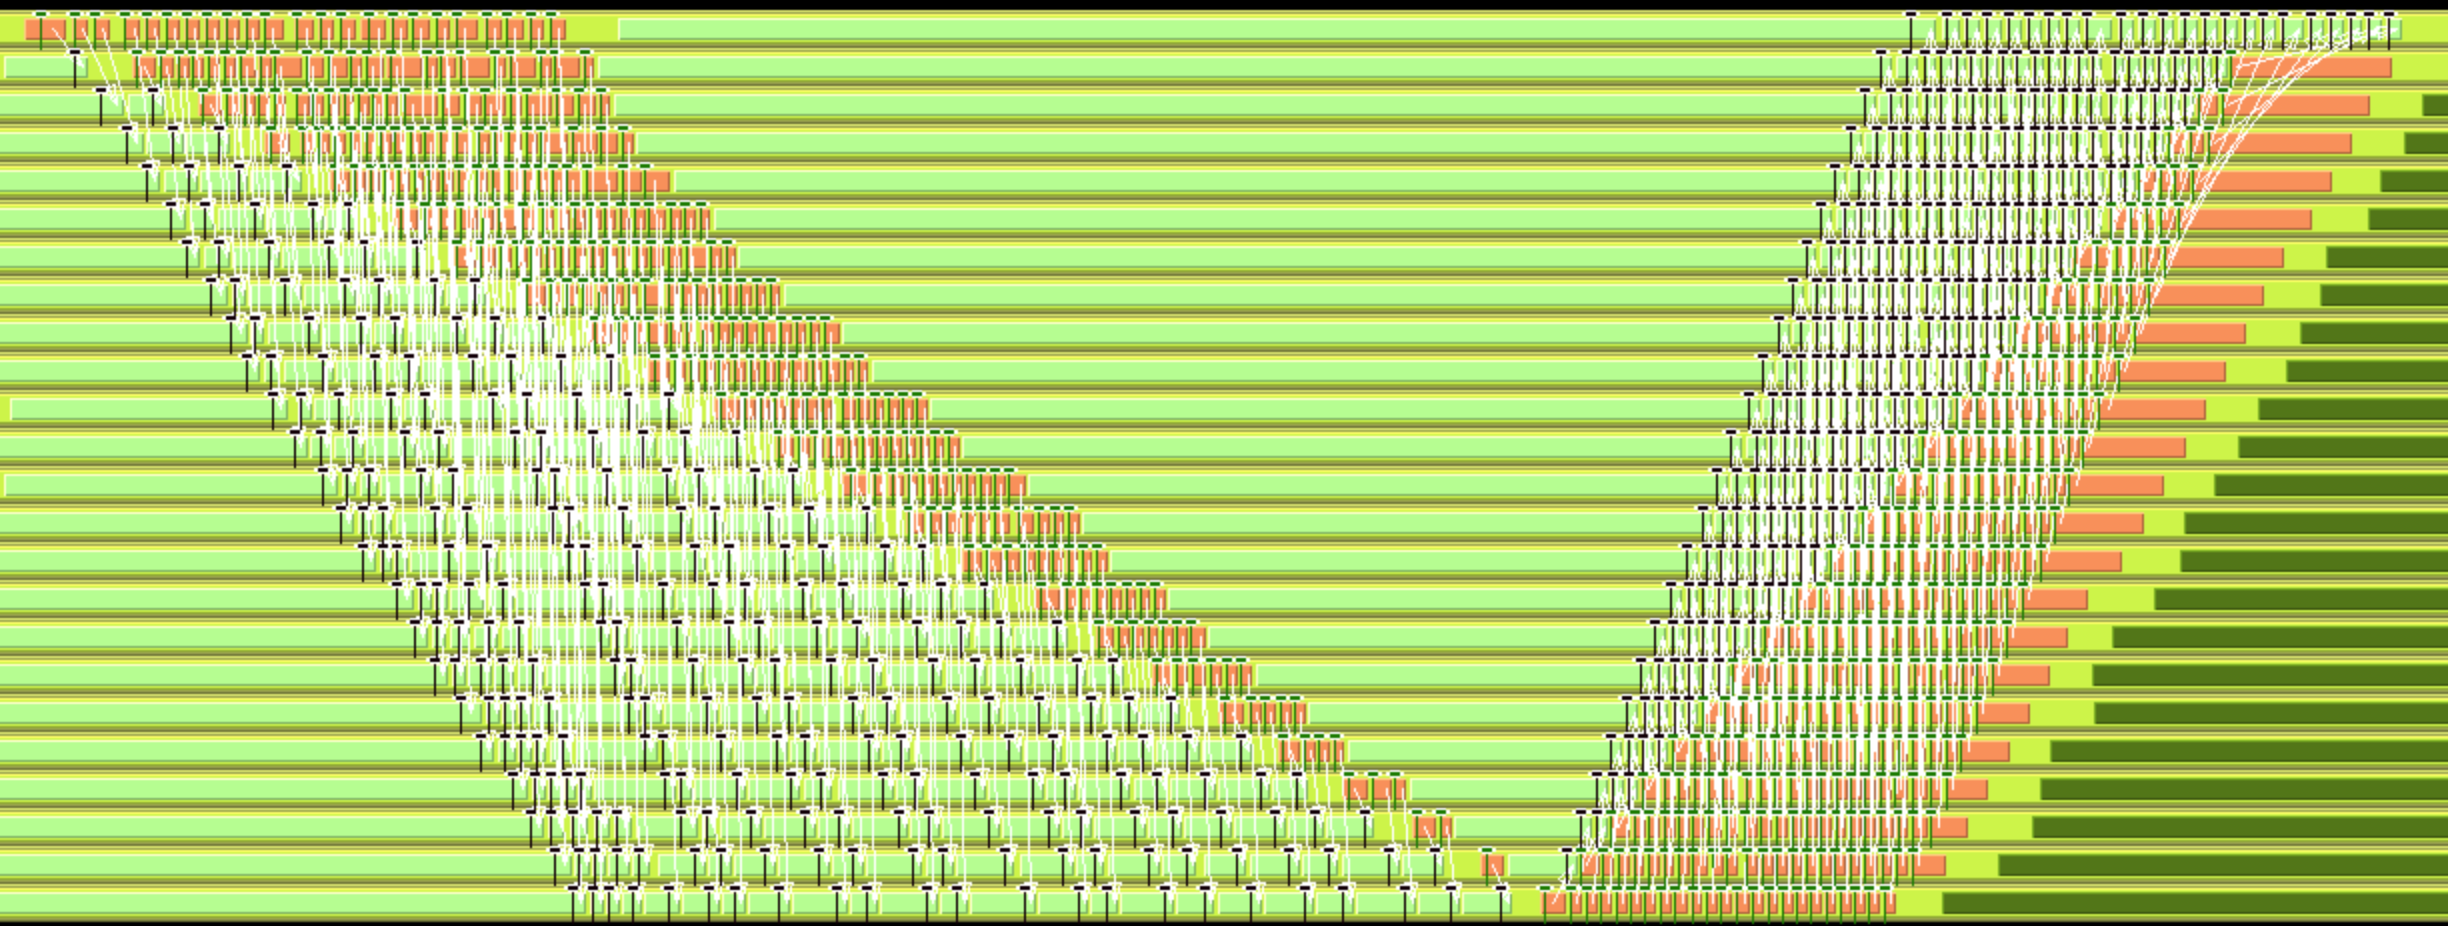
\includegraphics[scale=.3]{cascade}
\end{frame}

\begin{exerciseframe}[isendrecv]
  The proper solution is of course the use of \n{MPI_Irecv}.

  Make a TAU visualization of a run of \n{isendrev.c}.\\
  Is this optimal?
\end{exerciseframe}

\end{document}

%%%%
%%%% leftover exercises
%%%%

\begin{exerciseframe}[hang0]
  Each process iterates until it finds a small enough random.
  \begin{enumerate}
  \item \n{make hang0}
  \item \n{ddt hang0}
  \item Every process outputs a different value. Why?
  \item Use stepping or breakpoints
  \end{enumerate}
\end{exerciseframe}

\begin{exerciseframe}[hang1]
  \begin{enumerate}
  \item the author of \n{hang0.c} has attempted to fix the program
  \item \n{make hang1}
  \item in DDT: \n{File > New Session}
  \item run the program: only one process prints output.\\
    none of the processes finish.
  \item hit pause, check under `stacks' where the processes are
    hanging.
  \item set a breakpoint on the line where the return values are
    assigned, and rerun the program.
  \item fix the program
  \end{enumerate}
\end{exerciseframe}

\begin{exerciseframe}[broadcast]
  The author of \n{broadcast.c} was confused about the SPMD model.
  \begin{enumerate}
  \item The program as is will exit. Find the reason and fix.
  \item Now the program will hang. Find out why and fix it.
  \end{enumerate}
\end{exerciseframe}

\begin{exerciseframe}[ring]
  The author of \n{ring.c} has also misunderstood MPI. The goal of the
  program was to implement a send/recv around a ring, where every
  processors receives from its predecessor and successor.
  \begin{itemize}
  \item Run the program and see that the output is incorrect.
  \item Set a breakpoint on the send and receive
    statements. Rerun. What happens?
  \item Can you fix this program?
  \end{itemize}
\end{exerciseframe}

\begin{frame}[containsverbatim]{}
  \begin{itemize}
  \item 
  \end{itemize}
\end{frame}

